\item A small disc \( A \) is placed on an inclined plane forming an angle \( \alpha \) with the horizontal (Fig. 1.27) and is imparted an initial velocity \( v_0 \). Find how the velocity of the disc depends on the angle \( \varphi \) if the friction coefficient \( k = \tan \alpha \) and at the initial moment \( \varphi_0 = \pi/2 \).
    \begin{center}
        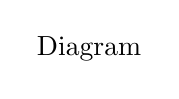
\begin{tikzpicture}
            \node at (0, 0) {Diagram};
        \end{tikzpicture}
    \end{center}
\begin{solution}
    \begin{center}
        \begin{tikzpicture}
            \pic at (0, 0) {frame=3cm};
        \end{tikzpicture}
    \end{center}
    
    \begin{align*}
        \intertext{The acceleration of the disk along the plane is determined by the projection of the force of gravity on this plane \(F_x = mg \sin \alpha\) and the friction force \(fr = kmg \cos \alpha\). In our case, \(k = \tan \alpha\) and therefore}
        fr &= F_x = mg \sin \alpha\\
        \intertext{Let us find the projection of acceleration on the direction of the tangent to the trajectory and on the \(x\)-axis}
        m w_t &= F_x \cos \varphi - fr = mg \sin \alpha \left( \cos \varphi - 1\right)\\
        m w_x &= F_x - fr \cos \varphi = mg \sin \alpha \left( 1 - \cos \varphi \right)\\
        \intertext{It is seen from this that \(w_t = - w_x\) which means that the velocity \(v\) and its projection \(v_x\) differ only by a constant value \(C\) which does not change with time, i.e.,}
        v &= -v_x + C,\ \text{where}\ v_x = v \cos \varphi.\ \text{The constant}\ C \ \text{is found from the initial condition}\,v=v_0, \, U_x = 0 \ \text{since}\, \varphi = \pi/2 \,\text{initially. Finally, we obtain}
        C &= v_0\\
        v &= \dfrac{v_0}{1+\cos \varphi}\\
        \intertext{In the course of time \(\varphi \to 0\) and \(v \to v_0/2\). (Motion then is unaccelerated.)}
    \end{align*}
\end{solution}
